\chapter{Spatial discretization and advection}\label{ch:adv}

This chapter describes how WRF discretizes the flux divergences of \cref{ch:eq}:
\begin{itemize}
  \item the staggered grid;
  \item the family of advection operators of orders 2 to 6;
  \item the positive-definite limiter for moisture and TKE.
\end{itemize}
The routines are in \code{dyn_em/module_advect_em.F}, which at about 13{,}000 lines is the largest file of the
dynamics.

\section{The C grid}

\begin{figure}[ht]
\centering
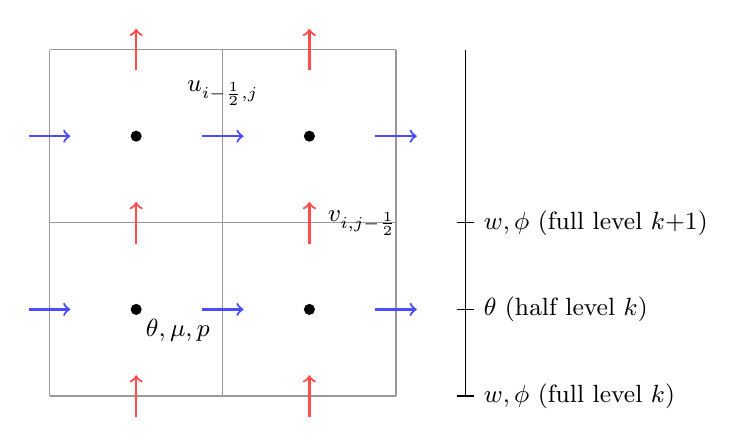
\begin{tikzpicture}[x=2.2cm,y=2.2cm]
  \draw[step=1, black!40] (0,0) grid (2,2);
  \foreach \x in {0.5,1.5} \foreach \y in {0.5,1.5} { \fill (\x,\y) circle (2pt); }
  \foreach \x in {0,1,2} \foreach \y in {0.5,1.5} { \draw[->, thick, blue!70] (\x-0.12,\y) -- (\x+0.12,\y); }
  \foreach \x in {0.5,1.5} \foreach \y in {0,1,2} { \draw[->, thick, red!70] (\x,\y-0.12) -- (\x,\y+0.12); }
  \node[below right] at (0.5,0.5) {\small $\theta, \mu, p$};
  \node[above] at (1,1.62) {\small $u_{i-\frac12,j}$};
  \node[right] at (1.55,1.0) {\small $v_{i,j-\frac12}$};
  \draw (2.4,0) -- (2.4,2);
  \foreach \y/\l in {0/{$w, \phi$ (full level $k$)}, 0.5/{$\theta$ (half level $k$)}, 1/{$w, \phi$ (full level $k{+}1$)}} {
    \draw (2.35,\y) -- (2.45,\y); \node[right, font=\small] at (2.45,\y) {\l};
  }
\end{tikzpicture}
\caption{The Arakawa C grid: horizontal plane (left) and the vertical staggering (right). Mass points (dots) hold
scalars; $u$ sits on the $x$-faces, $v$ on the $y$-faces; $w$ and $\phi$ on the full levels between half levels.}
\label{fig:cgrid}
\end{figure}

\Cref{fig:cgrid} shows the staggering. A grid cell $(i,j,k)$ has its mass point at the centre. $u_{i,j,k}$ in the
arrays is the value on the face at $i - \frac12$, $v_{i,j,k}$ the value at $j - \frac12$, and $w_{i,j,k}$ the value
on the full level below half level $k$. Averages to other positions are simple two-point means. For example, the
column mass at a $u$ point is $\frac12(\mu_{i-1,j} + \mu_{i,j})$, computed by
\src{dyn_em/module_big_step_utilities_em.F}{calc_mu_uv}.

\section{Flux-form advection}

For a scalar $q$ (or a velocity component), the advection term of \cref{eq:Q} in the $x$ direction is the
divergence of the flux $F = U q$ between faces:
\begin{equation}
  \bigl(m_x m_y\,\partial_x(Uq)\bigr)_{i} \approx m_x m_y\,\frac{F_{i+\frac12} - F_{i-\frac12}}{\Delta x} .
\end{equation}
Because the same face flux leaves one cell and enters its neighbour, the scheme conserves $\int \mu_d q$ exactly up
to round-off. The order of accuracy is set by how $q$ at the face is reconstructed from the cell values. With the
face at $i - \frac12$, the neighbours $q_{i-3}, \dots, q_{i+2}$, and the advecting velocity $u$ at the face, the
code's statement functions in \src{dyn_em/module_advect_em.F}{advect_scalar} are:
\begin{align}
  \mathrm{flux4} &= \frac{7\,(q_i + q_{i-1}) - (q_{i+1} + q_{i-2})}{12}, \label{eq:flux4}\\
  \mathrm{flux3} &= \mathrm{flux4} + \operatorname{sign}(u)\,
                    \frac{(q_{i+1} - q_{i-2}) - 3\,(q_i - q_{i-1})}{12}, \label{eq:flux3}\\
  \mathrm{flux6} &= \frac{37\,(q_i + q_{i-1}) - 8\,(q_{i+1} + q_{i-2}) + (q_{i+2} + q_{i-3})}{60}, \label{eq:flux6}\\
  \mathrm{flux5} &= \mathrm{flux6} - \operatorname{sign}(u)\,
                    \frac{(q_{i+2} - q_{i-3}) - 5\,(q_{i+1} - q_{i-2}) + 10\,(q_i - q_{i-1})}{60}. \label{eq:flux5}
\end{align}
The face flux is the coupled velocity times the reconstruction, for example
$F_{i-\frac12} = U_{i-\frac12}\;\mathrm{flux5}(q_{i-3}, \dots, q_{i+2}, u)$.
\begin{itemize}
  \item The even orders are centred.
  \item The odd orders add an upwind-biased term proportional to $|u|$ times a high-order derivative. That term is
    an implicit hyper-diffusion, which makes the odd orders the usual choice: fifth order horizontally and third
    order vertically (\code{h_mom_adv_order = 5}, \code{v_mom_adv_order = 3}, and the same for scalars).
\end{itemize}
The factor \code{sign(1,time_step)} in the code flips the upwind side for backward integration; for forward runs it
is $+1$.

\paragraph{Near the boundaries.} A fifth-order flux needs three cells on each side. Next to a specified or open
lateral boundary the stencil is not available, so the code lowers the order:
\begin{itemize}
  \item a second-order centred flux on the face next to the boundary;
  \item a third-order flux on the face after it;
  \item the full fifth-order flux from the fourth face inward.
\end{itemize}
Each of the three momentum routines and the scalar routine has this logic for every direction and boundary type. This
is why \code{module_advect_em.F} is long: the same stencil appears many times with different index ranges.

\paragraph{Vertical advection.} The vertical flux uses the same reconstructions in $\eta$, with $\Omega$ as the
advecting mass flux. It falls back to second order next to the surface and the top, and it is zero at both.

\section{Momentum advection}

$u$, $v$ and $w$ are advected by \src{dyn_em/module_advect_em.F}{advect_u}, \code{advect_v} and \code{advect_w}.
The advecting fluxes must be averaged to the faces of the momentum control volumes. For $u$, whose control volume is
centred on the $x$-face, the $x$-flux at its own centre uses $\frac12(U_{i} + U_{i+1})$. The $w$ equation has its
own control volumes centred on full levels, with an extra flux at the model lid.

\begin{algorithm}[ht]
\caption{The $y$-flux part of \code{advect_u} as written for a CPU (one $k$ level shown). The face flux of row $j$
is kept in a one-row buffer and reused as the lower flux of row $j+1$.}
\label{alg:advect-y}
\begin{algorithmic}[1]
\For{$j = j_{\mathrm{start}}, \dots, j_{\mathrm{end}}+1$} \Comment{faces of rows, in order}
  \For{$i$}
    \State $v_f \gets$ advecting $V$ averaged to the $u$ point at face $j$
    \State $F^{\mathrm{new}}_i \gets v_f \cdot \mathrm{flux5}(u_{i,j-3}, \dots, u_{i,j+2}, v_f)$ \Comment{or a lower order near a boundary}
  \EndFor
  \If{$j > j_{\mathrm{start}}$}
    \For{$i$}
      \State $T_{i,j-1} \gets T_{i,j-1} - m\,\frac{1}{\Delta y}\,(F^{\mathrm{new}}_i - F^{\mathrm{old}}_i)$
    \EndFor
  \EndIf
  \State $F^{\mathrm{old}} \gets F^{\mathrm{new}}$ \Comment{rolling buffer}
\EndFor
\end{algorithmic}
\end{algorithm}

\begin{portnote}
\Cref{alg:advect-y} carries a dependency from one $j$ row to the next through the buffer $F^{\mathrm{old}}$, so its
$j$ loop cannot run in parallel as written. The GPU version (Template B, kernels K-ADVU-Y1 and K-ADVU-Y2) splits it in
two:
\begin{enumerate}
  \item the first kernel computes every face flux into a three-dimensional work array;
  \item the second kernel forms the difference of two stored fluxes for every cell.
\end{enumerate}
Each flux is computed once with the same expression, and each tendency is updated with the same difference in the
same order, so the result is bitwise identical. The cost is one extra array write and read, which kernel fusion and
tiling later remove (\cref{ch:fusion,ch:tiling}).
\end{portnote}

\section{Positive-definite transport}

The odd-order schemes are not monotonic: near sharp gradients they can produce small negative mixing ratios. WRF's
positive-definite option (\code{moist_adv_opt = 1}, \code{tke_adv_opt = 1}) removes them in the last RK stage with a
flux limiter \citep{skamarock2009}, in \src{dyn_em/module_advect_em.F}{advect_scalar_pd}. Each face flux is split into a
first-order upwind part and a high-order correction:
\begin{equation}
  F = F^{\mathrm{L}} + F^{\mathrm{H}}, \qquad
  F^{\mathrm{L}}_{i-\frac12} = U_{i-\frac12}\,\bigl(q_{i-1}\ \text{if } U > 0,\ q_i \text{ otherwise}\bigr).
\end{equation}
The upwind update alone cannot create negative values when the Courant number is below 1. For each cell the limiter
computes:
\begin{itemize}
  \item the mass of the scalar that would remain after the low-order fluxes alone,
    \begin{equation}
      q^{\mathrm{low}} = \mu^{\mathrm{old}} q^{\mathrm{old}} - \Delta t\,\Bigl[m_x m_y\Bigl(\frac{\delta_x F^{\mathrm{L}}_x}{\Delta x}
                         + \frac{\delta_y F^{\mathrm{L}}_y}{\Delta y}\Bigr) + m_y\,\frac{\delta_\eta F^{\mathrm{L}}_\eta}{\Delta\eta}\Bigr] \ \ge 0;
    \end{equation}
  \item the mass the high-order corrections would carry out of the cell,
    \begin{equation}
      q^{\mathrm{out}} = \Delta t\,\Bigl[m_x m_y\Bigl(\frac{\max(0, F^{\mathrm{H}}_{i+\frac12}) - \min(0, F^{\mathrm{H}}_{i-\frac12})}{\Delta x} + \dots\Bigr) + \dots\Bigr].
    \end{equation}
\end{itemize}
If $q^{\mathrm{out}} > q^{\mathrm{low}}$, every \emph{outgoing} correction of that cell is multiplied by
$s = \max\bigl(0,\, q^{\mathrm{low}}/(q^{\mathrm{out}} + \epsilon)\bigr)$. The new value then follows from the
divergence of $F^{\mathrm{L}} + F^{\mathrm{H}}$.

\begin{algorithm}[ht]
\caption{The positive-definite limiter of \code{advect_scalar_pd}, as written for a CPU.}
\label{alg:pd}
\begin{algorithmic}[1]
\State compute $F^{\mathrm{L}}$ and $F^{\mathrm{H}} = F - F^{\mathrm{L}}$ on all faces (x, y, z)
\State compute $q^{\mathrm{low}}$ and $q^{\mathrm{out}}$ for all cells
\For{$j$, $k$, $i$ over the cells}
  \If{$q^{\mathrm{out}}_{ijk} > q^{\mathrm{low}}_{ijk}$}
    \State $s \gets \max(0, q^{\mathrm{low}}/(q^{\mathrm{out}} + \epsilon))$
    \State \textbf{if} $F^{\mathrm{H}}_{x,i+1} > 0$ \textbf{then} $F^{\mathrm{H}}_{x,i+1} \gets s\,F^{\mathrm{H}}_{x,i+1}$; \quad
           \textbf{if} $F^{\mathrm{H}}_{x,i} < 0$ \textbf{then} $F^{\mathrm{H}}_{x,i} \gets s\,F^{\mathrm{H}}_{x,i}$
    \State the same for $y$; for $z$ with the signs reversed ($\eta$ decreases upward)
  \EndIf
\EndFor
\State update: divergence of $F^{\mathrm{L}} + F^{\mathrm{H}}$
\end{algorithmic}
\end{algorithm}

\begin{portnote}
In \cref{alg:pd} a face is shared by two cells, and the CPU loop visits the cells in order. A face can therefore be
scaled by its upwind donor cell in one iteration and read by its other neighbour in the next. A naive parallel loop
over cells would let two threads touch the same face: a data race, and a result that depends on scheduling.

The port splits the limiter (kernels K-PD-L3a and K-PD-L3b):
\begin{enumerate}
  \item one kernel computes the factor $s$ of every cell, or a sentinel for ``not limited'';
  \item one kernel per direction visits every face once and applies the factor of the face's donor cell, by exactly
    the rules of the source, including zero fluxes and the edges of the loop range.
\end{enumerate}
Each face is scaled at most once, by the same factor the CPU applies, so the result is identical. The unit test
T-PDLIM proves it on random and real states (\cref{ch:subsys}).
\end{portnote}

\section{Other options}

\begin{description}
  \item[Monotonic transport] (\code{moist_adv_opt = 2}) adds a second limiter that keeps the new value within the
    range of its upwind neighbours.
  \item[WENO] (\code{moist_adv_opt = 3, 4}) replaces the fixed stencils by weighted essentially non-oscillatory
    reconstructions of fifth order.
  \item[Even orders] (\code{h_*_adv_order = 4, 6}) are available but rarely used, because they need explicit
    diffusion.
\end{description}
The case uses none of these, so the port leaves them on the CPU and its startup check rejects them (\cref{ch:case}).
